\documentclass[a4paper,10pt]{article}
\usepackage{hyperref}
\usepackage{float}
\usepackage{graphicx}

%%% Title
\title{Processo e Sviluppo Software: Assignment 3} 
\author{Ivo Junior Bettini - 806878, Umberto Cocca - 807191, \\Silvia Traversa - 816435\\
\href{https://gitlab.com/s.traversa/2019_assignment3_booksloan}{GitLab repository}}
\date{}

\begin{document}

\maketitle 


\section*{Applicazione BooksLoan}
L'applicazione proposta permette agli utenti di visualizzare il catalogo di una biblioteca. Essi possono visualizzare sia le copie disponibili, ed eventualmente richiederne una in prestito, sia quelle non disponibili e prenotarle per quando ritorneranno presso la biblioteca.
E' inoltre possibili visualizzare le informazioni relative ad ogni singolo libro, quali l'autore o la presenza di sequel. 

\section*{Schema E-R}

\begin{figure}[H]
	\centering
	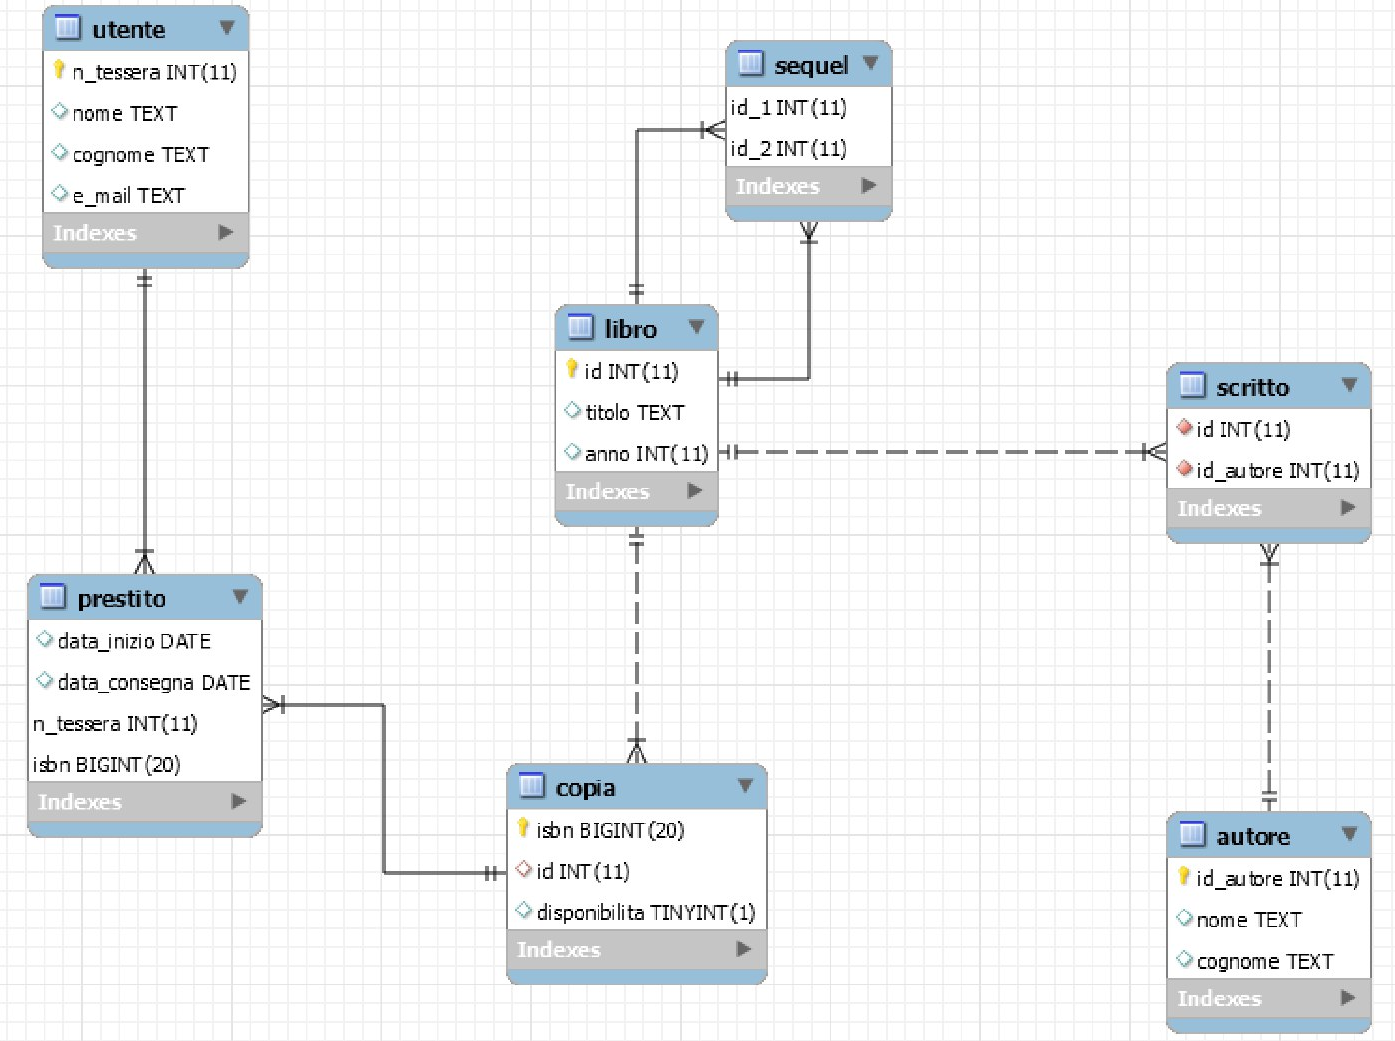
\includegraphics[width=0.7\linewidth]{images/ERdiagram}
	\caption[Schema ER]{Schema ER}
	\label{fig:re}
\end{figure}

\begin{itemize}
	\item Un utente può richiedere in prestito una sola copia di un libro
	\item Un libro può essere presente in più copie o nessuna
	\item Una copia può trovarsi in due stati, disponibile o non
	\item Un libro può essere collegato ad un altro in quanto suo sequel
	\item Un libro può essere scritto da uno o più autori e un autore può scrivere uno o più libri
\end{itemize}

\end{document}
